% File: stack.tex
% Description: A hardcoded TikZ stack - not generic, not scalable at all.

\documentclass{standalone}
\usepackage{xcolor}
\usepackage{amsmath}
\usepackage{tikz}
\usetikzlibrary{chains}
\usetikzlibrary{calc}
\usetikzlibrary{shapes}
\usetikzlibrary{arrows.meta}

\definecolor{alacenaOrange}{HTML}{CFB267}
\definecolor{alacenaTurquoise}{HTML}{5480B5}
\definecolor{alacenaBlue}{HTML}{3D619D}

\newcommand\nn[1]{\text{\textup{\textbf{\texttt{#1}}}}}

\begin{document}

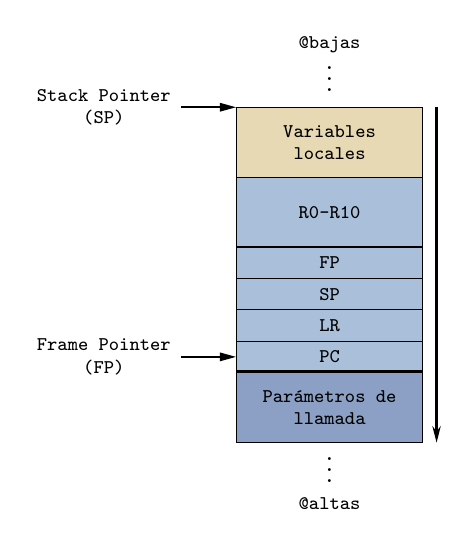
\begin{tikzpicture}
    \begin{scope}[start chain=going left, node distance=0pt]
        \tikzstyle{frame} = [
            font=\scriptsize,
            draw,
            on chain,
            rectangle split,
            rectangle split parts=20,
            % rectangle split part align={center, left},
            rectangle split empty part height = 0ex,
            rectangle split empty part depth = 0ex,
            rectangle split empty part width = 0ex,
        ]
        
        \node (main) [
            frame,
            rectangle split parts=7,
            rectangle split part fill = {
                alacenaOrange!50,
                alacenaTurquoise!50,
                alacenaTurquoise!50,
                alacenaTurquoise!50,
                alacenaTurquoise!50,
                alacenaTurquoise!50,
                alacenaBlue!60
            } 
        ] { %
        \nodepart{one} \parbox[c][6ex]{20ex}{\centering \nn{Variables}\\ \nn{locales}}
        \nodepart{two} \parbox[c][6ex]{20ex}{\centering \nn{R0-R10}}
        \nodepart{three} \nn{FP}
        \nodepart{four} \nn{SP}
        \nodepart{five} \nn{LR}
        \nodepart{six} \nn{PC}
        \nodepart{seven} \parbox[c][6ex]{20ex}{\centering \nn{Parámetros de}\\ \nn{llamada}}
        };

        \draw[very thick]
            ($(main.north west) + (0,-22.2ex)$) --
            ($(main.north east) + (0,-22.2ex)$);

        \draw[-{Stealth[length=6pt, width=3pt]}, thick]
            ([xshift=5pt]main.north east) -- 
            ([xshift=5pt]main.south east);

        \draw[-{Triangle[length=6pt, width=3pt]}, thick]
            ([xshift=-20pt]main.north west) -- 
            (main.north west)
            node[left=10pt, midway, font=\scriptsize, align=center] {\texttt{Stack Pointer} \\ \texttt{(SP)}};

        \draw[-{Triangle[length=6pt, width=3pt]}, thick]
            ([xshift=-20pt]main.six west) -- 
            (main.six west)
            node[left=10pt, midway, font=\scriptsize, align=center] {\texttt{Frame Pointer} \\ \texttt{(FP)}};

        \node[above=0.5ex of main.north, align=center] (dotsTop) {
            \scriptsize \texttt{@bajas}\\[-0.5ex]
            $\vdots$
        };

        \node[below=-1ex of main.south, align=center] (dotsBottom) {
            $\vdots$ \\[-0.5ex]
            \scriptsize \texttt{@altas}
        };
    \end{scope}
\end{tikzpicture}

\end{document}
